\documentclass[12pt,a4paper]{article}

\usepackage[utf8]{inputenc}
\usepackage[T1]{fontenc}
\usepackage{array}
\usepackage{booktabs}
\usepackage{multirow}
\usepackage{titlesec}
\usepackage{tocbibind}
\usepackage{tocloft}
\usepackage{graphicx}
\usepackage{caption}
\usepackage{float}
\usepackage{indentfirst}
\usepackage{setspace}
\usepackage[backend=biber, style=numeric, sorting=none]{biblatex}
\addbibresource{references.bib}

\titleformat{\section}{\normalfont\Large\bfseries}{第\ \thesection 章}{1em}{}
\setcounter{tocdepth}{2}
% "Contents" を "目次" に変更
\renewcommand{\contentsname}{目次}

% 図のキャプションを「Figure」から「図」に変更
\captionsetup[figure]{labelformat=simple, labelsep=space, name=図}
\captionsetup[table]{name=表}

\begin{document}
\onehalfspacing


\begin{titlepage}
\centering
\vspace*{60pt}
{\Large 令和5年度 卒業研究論文}\\[50pt]
{\Large \textbf{カーレースゲームを用いた深層強化学習による\\安全運転の設計と開発}}\\[120pt]
{\Large 電子情報工学科}\\[50pt]
{\Large 学生氏名 レオラ デイビット\\指導教員 越野 亮}\\[50pt]
{\Large 令和6年2月20日 提出}
\end{titlepage}

\newpage
\section*{要旨}
世界の多くの国々,特に発展途上国では,車やバイクが非常に多いが,交通ルールがしっかり守られていないことがよくある.この問題は,交通のインフラが十分でないことや,交通法規を厳しく守ることが不足しているために起きている.これにより,混雑した道路での危険な運転行動が増え,交通事故のリスクが高まっている.

特に,速く運転することは非常に危険である.速い速度で運転すると,反応時間が短くなり,予期せぬ障害物に対処する能力が低下する.これは,事故が起きた時に,より深刻な結果を招く原因となる.車やバイクが多く,安全対策が不十分で,速く運転する人が多いことが,交通事故を引き起こす大きな原因となっている.そのため,より良い道路のインフラを整えること,法律を厳しく守ること,そして,安全運転についての意識を高めることが重要である.


\section*{Abstract}
In many developing countries, the sharp increase in cars and motorcycles outpaces the enforcement of traffic regulations, leading to hazardous road conditions. Often, this problem stems from inadequate transportation infrastructure and poor traffic law enforcement, which allows dangerous driving behaviors to proliferate, especially in congested areas. This situation increases the risk of accidents, particularly at high speeds, which reduces a driver's reaction time and makes it harder to avoid sudden obstacles, leading to more severe accidents. The combination of high vehicle density, insufficient road safety measures, and a tendency towards speeding creates a high risk for traffic incidents. This underscores the urgent need for comprehensive road safety strategies that include improved infrastructure, stricter law enforcement, and increased public awareness of safe driving practices.

\newpage
\addtocontents{toc}{\protect\setcounter{tocdepth}{-1}}
\tableofcontents
\addtocontents{toc}{\protect\setcounter{tocdepth}{2}}

\newpage
\section{はじめに}
深層強化学習は,Atari,Go,StarCraft,DOTAといった分野で最近の印象的な人工知能の成果の鍵となっている.深層強化学習がロボティクスや自動化に影響を与えるためには,複雑な物理システムの制御における成功を示す必要がある.また,ロボティクスの多くの潜在的な応用は,人間の近くで相互作用し,不正確に指定された人間の規範を尊重しながら行うことを要求する.カーレースは,これらの課題を正確に提起するドメインであり,複雑で非線形なダイナミクスを持つ車両をリアルタイムで制御し,対戦相手の数インチ以内で運用することを要求する.幸いなことに,このドメインには非常に現実的なシミュレーションが存在し,機械学習アプローチの実験に適している\cite{Gran-Turismo-Sophy}.

本研究では Unity を用いてゲーム環境を開発し,深層強化学習を用いてカーレースAIの学習を行っている.この試みは,交通事故における対応策,特に予測できない運転行動への対応として,自動運転技術の発展を目指している.訓練されたAIエージェントは,様々な交通状況下での適切な反応と安全運転技術を学習する.


\newpage
\section{強化学習の基本と初期の学習アプローチ}
本章では,本研究において採用された強化学習および適用された学習手法について説明する.さらに,参照したGitHub上のカーレースAIサンプルおよびその成果と課題についても開設する.
\subsection{強化学習の基礎と学習サイクル}
強化学習(Reinforcement learning)は,エージェントが環境の状態を観察し,どのように行動すれば最大の報酬を獲得できるかを学習する手法である.強化学習のサイクルは以下のように進行する.
\begin{enumerate}
  \item 状態取得:エージェントは環境を観察し,その状態を取得する.
  \item 行動決定:エージェントは,観察した状態に基づいてポリシーに従って行動を決定する.
  \item 行動実行:エージェントは,決定された行動を実行する.
  \item 報酬取得:行動の結果として,エージェントは報酬を受け取る.
  \item ポリシー更新:獲得した報酬と経験に基づき,ポリシーを更新する.
\end{enumerate}

最終的に,エージェントはこのサイクルを繰り返し,将来的に多くの報酬を得るためのポリシーを見つけ出す.

\subsection{エージェントの行動タイプ} 
強化学習サイクルでは,エージェントは取得した環境の状態に応じてエージェントが行動を選択する.行動には,連続値(Continuous)と離散値(Discrete)の2つの型がある.「Continuous」の場合,-1.0 から 1.0のような連続した値を取る浮動小数点数の配列を行動として使用する.一方,「Discrete」の場合は,0,1,2 のような離散した値を持つ整数配列を行動として使用する.本研究で使用したGitHubのカーレースAIサンプルでは「Continuous」型の行動が採用されているが,第3章「スクラッチから学習環境の構築」では,「Discrete」型の行動を用いた.サンプルのカーレースAIの実装結果に基づき,「Continuous」型では浮動小数点数を用いるため操作の選択肢が非常に多く,初期段階で経験のないエージェントにとって学習が難しく,失敗する可能性が高かまる.一方で,「Discrete」型では離散が限られているため,エージェントの学習を容易に進めることが可能になる.

\subsection{使用した学習手法}
Unity ML-Agentsでは,「PPO」と「SAC」の2つの強化学習アルゴリズムが利用可能である.ハイパーパラメータの設定項目は,使用するアルゴリズムが「SAC」か「PPO」かによって異なる.
「SAC」(Soft Actor-Critic)はオフポリシーのアルゴリズムであり,過去の経験から学習を促進する.一方,「PPO」(Proximal Policy Optimization)はオンポリシーのアルゴリズムで,現在のポリシーに基づいて学習を進める.PPOは,学習過去の安定性を高めるために,ポリシーの急激な変更を抑制する特徴がある.
本研究では,カーレースAIのサンプルおよびスクラッチから構築した学習環境において,「PPO」アルゴリズムを用いて学習を行った.

\subsection{エージェントの環境認識:観察とセンサー}
カートの学習において,初期段階ではカートがランダムに動きながらトラックを探索する.この探索は,カメラではなく,周囲の環境を認識するためにRaycast 3D センサーを使用した.Unityでは,2Dおよび3Dの環境で使用可能なRaycastセンサーがあるが,本研究では3Dの環境で学習を行うため,Raycast 3D センサーを使用した.

\subsection{エージェントクラスのオーバーライドメソッド}
エージェントのスクリプトでは,エピソード開始時の初期化,観察の取得,行動の実行と報酬の取得などを実装する.以下に,本研究で使用されたいくつかの重要なエージェントクラスを説明する.
\begin{enumerate}
  \item \textbf{OnEpisodeBegin() の追加:}エピソードが開始する際に実行される関数である.
  \item \textbf{CollectObservations() の追加:}エージェントが観察を収集する関数である.引数 'VectorSensor' の 'AddObservation()' メソッドを使用して,観察の値をエージェントに渡す.
  \item \textbf{OnActionReceived() の追加:}決定された行動に基づいて行動を実行する.
\end{enumerate}

この3つのメソッドは,学習用スクリプトを作成する際に特に重要視された.また,これらの設定に関する詳細は,後述の「サンプルの実行の詳細」と「学習用のエージェントスクリプト」のセクションで説明される.

\subsection{サンプル実行の詳細}
\subsubsection{サンプルの学習環境}
カーレースゲームのサンプルは,GitHubで公開されているレーシングゲームのサンプル\cite{AI-Racing-Karts}を基にしている.
学習の初期段階では,公開されているトラックを使用し,カートを配置して学習を開始した.学習プロセスを高速化するために,複数のカートをトラック上に配置した.

また,使用したカーレースAIサンプルの学習環境におけるトラックレイアウトやカートのモデルを,図1と図2に示す.

\begin{figure}[H]
    \centering
    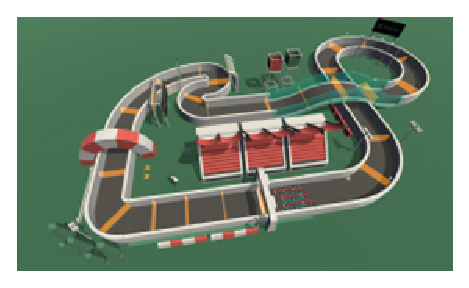
\includegraphics[width=0.8\textwidth]{figures/TrackLayout.eps}
    \caption{カーレースAIサンプルの学習環境【トラックのレイアウト】}
    \label{fig:sample-environment}
\end{figure}

\begin{figure}[H]
    \centering
    \includegraphics[width=0.8\textwidth]{figures/KartModel.eps}
    \caption{カーレースAIサンプルの学習環境【カートのモデル】}
    \label{fig:kart-model}
\end{figure}

\subsubsection{学習用のスクリプト}
カートを動かすためのスクリプトに加えて,学習するためのエージェントスクリプトが追加された.このスクリプトには,エージェントが行う行動に対して報酬の設定を追加した.行動のタイプは「Continuous」に設定された.これは,浮動小数点数を使用することでカートの動きをより滑らかに制御できるためである.報酬の設定では,トラック上に見えないチェックポイントを配置し,これを正しく通過すると報酬が与えられる.また,カートが誤ったチェックポイントを通過するとペナルティとしてマイナスの報酬を与えるように設定された.学習プロセスを効率的に進めるため,20ms ごとに小さなマイナスの報酬を適用した.

Unity ML-Agentsを用いた学習プロセスは,'mlagents-learn' コマンドと学習設定ファイルを使用して行われる.このプロセスを通じて,コマンドライン引数と学習設定ファイルのパラメータに基づいて学習が実施される.

\subsubsection{学習結果と考察}
カーレースAIサンプルの学習結果はTensorboardで閲覧することができ,累計報酬とエピソードの長さの詳細が確認できる.その学習結果を以下の図3に示す.

\begin{figure}[H]
    \centering
    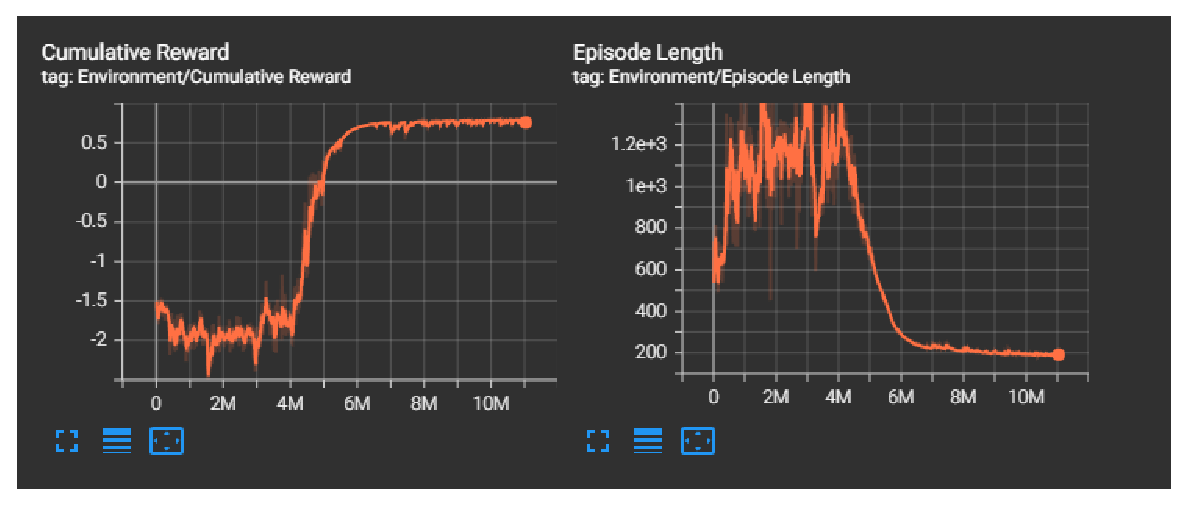
\includegraphics[width=1\textwidth]{figures/Tensorboard.eps}
    \caption{カーレースゲームサンプルの結果}
    \label{fig:sample-graph}
\end{figure}


図3からわかるように,400万ステップの学習を実施した結果,初期は累計報酬がマイナスであったものの,250万ステップ目以降に累計報酬が著しく向上した.報酬の向上に伴い,エピソードの長さも短縮されていることが確認できた.

しかし,この学習結果にはいくつかの問題点があった.学習の初期段階では,カートが後退し続けることで累計報酬が改善されず,学習プロセスを何度も中断せざるを得なかったこと,カートの動きが現実の車とは異なり,停止状態でも左右に回転できるため不自然であったこと,そしてカートが壁に衝突する問題があったことである.壁に衝突した際のペナルティが導入されていなかったため,カートが壁を利用して前進し続けた.結果として,カーレースAIのサンプルでは壁に衝突せずに走行することは実現できなかった.

上記の問題点をすべて改善するため,スクラッチから新しい学習環境を構築することにした.この新しい学習環境,その構築過程,および学習結果については,以下の第3章以降で詳しく説明する.


\newpage
\section{実験方法}
カーレースAIのサンプルを改善するために,車の操作用のスクリプトからトラックやチェックポイントまで全てを変更する必要があるので,スクラッチから新しい車エージェントや環境を作成することがより効率的だと判断した.以下では,スクラッチからの環境構築プロセスについて説明する.
この章では,カリキュラム学習のアプローチを用いて学習を進めた.カリキュラム学習は,学習期間の短縮やモデルの精度向上のために,段階的に難易度を上げる手法である.

\subsection{道路の環境構築}
Unityのアセットストアから無料のシティ(City)モデルやスポーツカー(Sports Car)モデルをダウンロードした.
新しい道路のシンプルなレイアウトを作成し,手に入れたモデルをエディタ内に配置した.モデルを配置する際,学習時に問題が生じないようにモデルのサイズや位置を正確に設定した.新しい道路の壁には凸凹があったため,道路上に見えない直方体を作成し,壁を滑らかにした.滑らかにした状態を以下の図4に示す.
\begin{figure}[H]
    \centering
    \includegraphics[width=0.8\textwidth]{figures/invisible-wall.eps} % ここで図のファイル名とサイズを指定します
    \caption{滑らかにした道路の壁} % 図のキャプション
    \label{fig:invisible-wall} % 図への参照用ラベル
\end{figure}

\subsubsection{チェックポイントの配置}
新しい道路完成後,トラック上に56個の見えないチェックポイントを配置した.どのチェックポイントを通過したかを追跡するために,チェックポイント管理システムのスクリプトを作成し,それを各チェックポイントに付けた.このシステムでは,車が特定のチェックポイントを通過すると,そのチェックポイントのタグをシステムに更新する.全てのチェックポイントを通過した後,チェックポイントのタグはリセットされる.シチモデルと配置したチェックポイントの様子を以下の図5に示す.
\begin{figure}[H]
    \centering
    \includegraphics[width=0.8\textwidth]{figures/checkpoints.eps} % ここで図のファイル名とサイズを指定します
    \caption{配置されたチェックポイント} % 図のキャプション
    \label{fig:checkpoints} % 図への参照用ラベル
\end{figure}


\subsection{車エージェントの作成}
アセットストアからダウンロードしたモデルに適切なボディとタイヤのコライダーを設定し,モデルに合わせた.また,車モデルにリジッドボディ(Rigidbody)を付けて重力を受けるように設定した.リジッドボディとは,ゲームオブジェクトを物理特性によって制御することができるようにするコンポネントである.作成した車エージェントのモデルを以下の図6に示す.
\begin{figure}[H]
    \centering
    \includegraphics[width=0.8\textwidth]{figures/car1.eps} % ここで図のファイル名とサイズを指定します
    \caption{車エージェントのモデル} % 図のキャプション
    \label{fig:car-model} % 図への参照用ラベル
\end{figure}


\subsubsection{エージェントの Raycast 3D センサーの設定}
車が周囲の環境を正確に認識できるように,2種類の Raycast 3D センサーを設定した.1つ目のセンサーは車の前半部分の約180度にわたり15本のセンサーで,近くの壁やチェックポイントを識別する.作成した1つ目のセンサーとその設定を図7,図8に示す.\\
\begin{figure}[H]
    \centering
    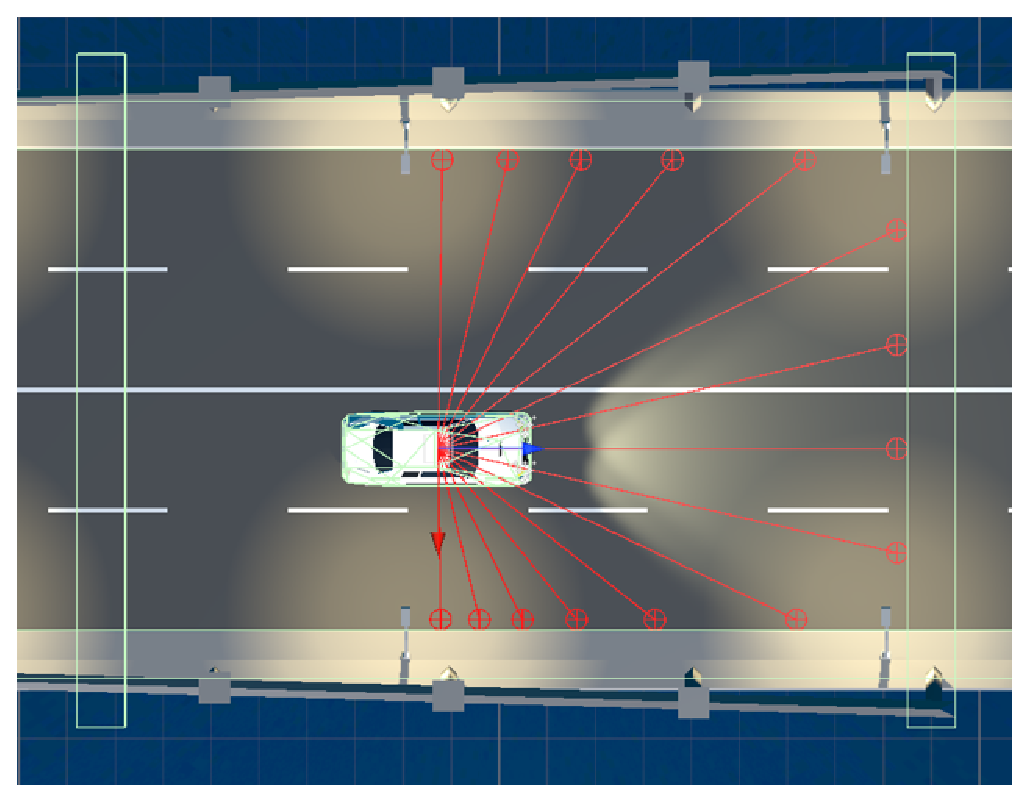
\includegraphics[width=0.8\textwidth]{figures/FirstRaycast.eps} % ここで図のファイル名とサイズを指定します
    \caption{1つ目のRayCastセンサー} % 図のキャプション
    \label{fig:first-raycast} % 図への参照用ラベル
\end{figure}

\begin{figure}[H]
    \centering
    \includegraphics[width=0.8\textwidth]{figures/FirstRaycastSettings.eps} % ここで図のファイル名とサイズを指定します
    \caption{1つ目のRayCastセンサーの設定} % 図のキャプション
    \label{fig:first-raycast-settings} % 図への参照用ラベル
\end{figure}

2つ目のセンサーは車の前方約90度にわたり13本のセンサーで,遠くの壁や障害物を識別する.これにより,車がスムーズに道路を進めるように各センサーがそれぞれの役割を果たす.作成した2つ目のセンサーとその設定を図9,図10に示す.
\begin{figure}[H]
    \centering
    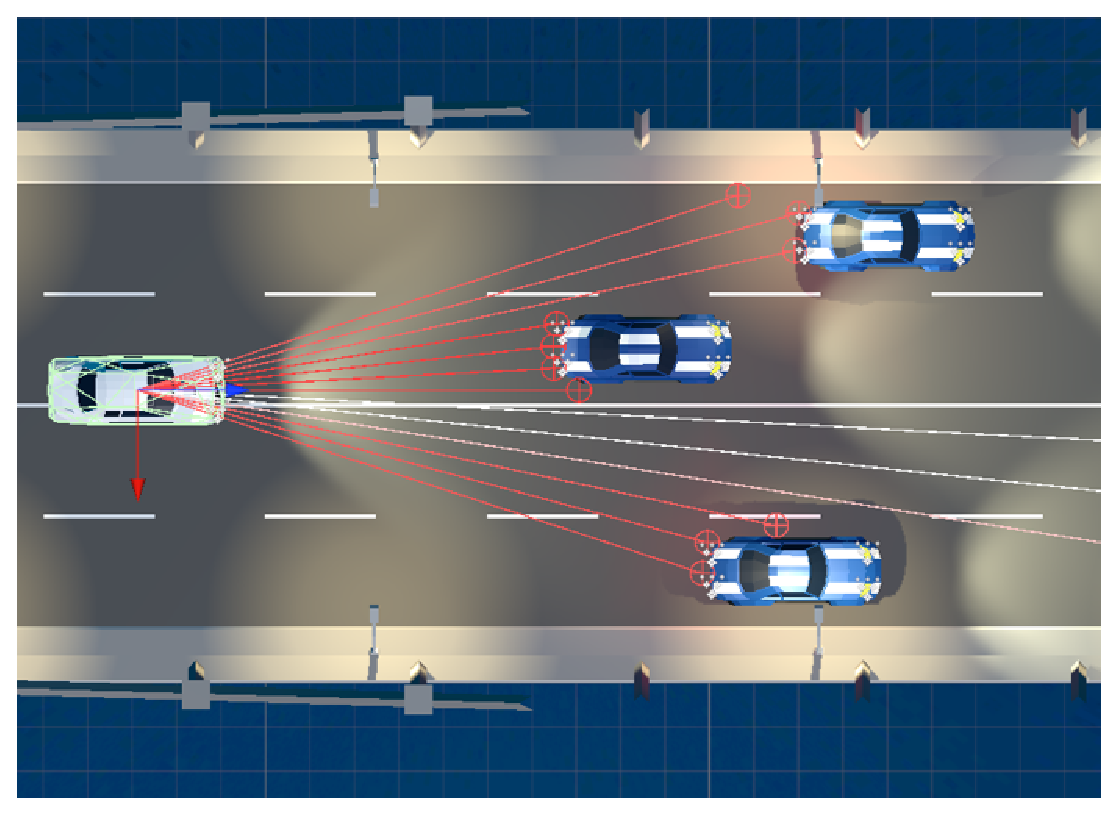
\includegraphics[width=0.8\textwidth]{figures/SecondRaycast.eps} % ここで図のファイル名とサイズを指定します
    \caption{2つ目のRayCastセンサー} % 図のキャプション
    \label{fig:second-raycast} % 図への参照用ラベル
\end{figure}

\begin{figure}[H]
    \centering
    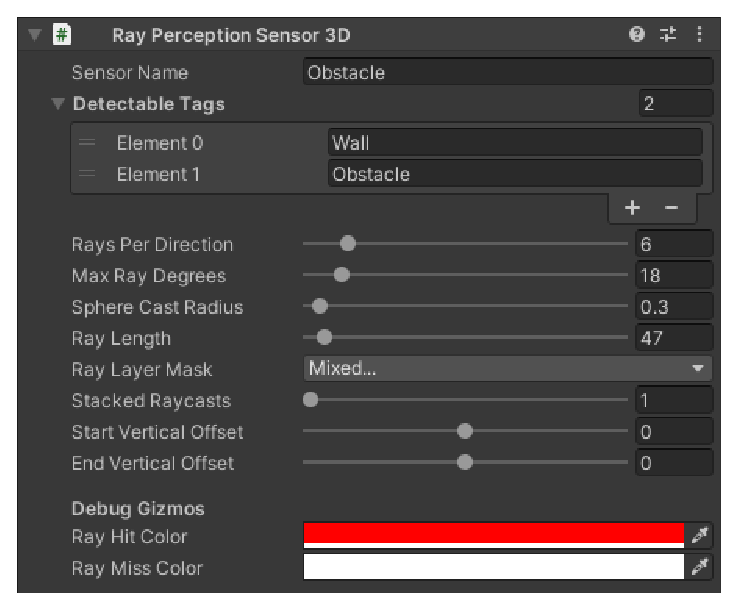
\includegraphics[width=0.8\textwidth]{figures/SecondRaycastSettings.eps} % ここで図のファイル名とサイズを指定します
    \caption{2つ目のRayCastセンサーの設定} % 図のキャプション
    \label{fig:second-raycast-settings} % 図への参照用ラベル
\end{figure}

\subsubsection{操作用のスクリプト}
エージェントに与えられた基本操作はアクセル,ブレーキ,および左右のステアリングである.ブレーキに関しては,通常のレーシングゲームでは完全に停止すると後退し始めるが,本研究ではハンドブレーキのように設定し,速度がゼロになると車は動かなくなるようにした.これは,学習中に車が不必要に後退することを防ぐためである.

\subsubsection{学習用のエージェントスクリプトの詳細}
学習プロセスを最適化するために,エージェントスクリプトでは様々なシナリオでの報酬とペナルティが設定されている.これにより,車エージェントは効率的に適切な行動を学習し,不適切な行動を避けることができる.
\begin{enumerate}
  \item OnEpisodeBegin()では,各エピソード開始時に車と障害物の位置と速度をリセットし,前のエピソードからの影響を排除する.これにより,エージェントが新しいエピソードでスムーズな状態から始めることができる.
  \item CollectObservations()では,エージェントは自信の位置や速度および次のチェックポイントの位置情報を収集する.これらの情報を基にエージェントは次の行動を決定する.
  \item OnActionReceived()では,エージェントの行動に基づいて報酬やペナルティが与えられる.これにより,エージェントは有益な行動を強化し,不利益な行動を避けるように学習する.
\end{enumerate}

\subsection{報酬システムの詳細}
\subsubsection{報酬(Reward)}
\begin{enumerate}
  \item \textbf{速度維持報酬:}
エージェントが一定の速度基準を超えると,小さな報酬(+0.0001f)が与えられる.これは車に速い走行を促すためである.
  \item \textbf{チェックポイント通過報酬:}
車が道路上に配置された見えないチェックポイントを通過するたびに,より大きな報酬(+0.5f)が与えられる.
\end{enumerate}

\begin{figure}[H]
    \centering
    \includegraphics[height=0.4\textheight]{figures/CheckpointReward.eps} % ここで図のファイル名とサイズを指定します
    \caption{チェックポイントを通過する度の報酬} % 図のキャプション
    \label{fig:checkpoint-reward} % 図への参照用ラベル
\end{figure}

\subsubsection{罰(Penalty)}
\begin{enumerate}
  \item \textbf{一定のペナルティ:}車には1ステップごとに(1ステップ=20ms)小さなペナルティ(-0.0001f)が与えられる.これは車が停止し続けるとペナルティが加算されるため,車が動き続けるように促すためである.
  \item \textbf{原則ペナルティ:}車が減速して速度がゼロになった場合は,車にペナルティ(-0.5f)が与えられ,車の状態がリセットされる.
  \item \textbf{学習難易度に応じて衝突したペナルティの調整:}壁や障害物に衝突した場合,学習の初期モデルでは小さめなペナルティを設定し,難易度が上がるにつれてペナルティ(-0.5fから-2.0fまで)増加させる.車が障害物に衝突した様子を図12に示す.
\end{enumerate}

\begin{figure}[H]
    \centering
    \includegraphics[height=0.4\textheight]{figures/CarCollision.eps} % ここで図のファイル名とサイズを指定します
    \caption{衝突した様子} % 図のキャプション
    \label{fig:car-collision} % 図への参照用ラベル
\end{figure}

\subsection{障害物の作成と操作スクリプト}
障害物(他車)はルールベースのAIによって制御され,指定された車線(レーン)を走行する.このAIは,レーン内の特定のインデックスを追跡し,それに従って移動する.レーンの作り方は次に説明する.

\subsection{車線(レーン)の作成}
本研究では,作成した道路環境の中に4つの車線が存在する.これらの車線は,障害物(他車)が指定されたレーンを走行するために必要である.各レーンは配列として機能し,指定されたレーンのすべての特定の位置が記録されている.\\

\noindent 車線(レーン)の作成方法:
\begin{enumerate}
  \item まず,4つの空のゲームオブジェクトを作成し,それぞれをファーストレーン(1st Lane),セカンドレーン(2nd Lane),サードレーン(3rd Lane),フォースレーン(4th Lane)と名付ける.
  \item 各レーンに50個以上の空のゲームオブジェクトを1周にわたって間隔を空けて適切に配置する.
  \item これらをレーンの配列に子オブジェクトとしてインデックス付けする.
  \item この手順を残りのレーンに対しても同様に行い,全てのレーンを作成する.
\end{enumerate}

続いて,各レーンの子オブジェクトのインデックスを追跡し,更新できるようにするため,レーンシステムを障害物を操作するスクリプトに組み込んだ.また,一方通行と対面通行の2つのモードを設定し,必要に応じてどちらかを選択できるようにした.さらに,1周にわたって各障害物(合計11台)のスポーンポイントを設定し,障害物が重ならないように設定した.

一方通行の場合は,すべての障害物を一方通行モードに設定して学習を進める.対面通行の場合は,日本の交通ルールに合わせて左車線を使用する.そのため,ファーストレーンとセカンドレーンの障害物はそのままにし,サードレーンとフォースレーンの障害物を対面通行モードに設定する.これにより,四車線での対面通行シナリオも学習できるようになる.




\newpage
\section{学習過程}
本章では,Unity ML-Agentsを用いた車エージェントの学習プロセスについて詳しく記述する.
\subsection{基本操作の学習}
エージェントは,初期段階で車の基本的な操縦技術を身につける.これには,加速,減速,方向転換といった基本的な車両操作の理解と,これらの操作を組み合わせて車両をコントロールする訓練が含まれる.報酬システムを通じて,エージェントは道路を無事に一周することで基本的な車両制御スキルを獲得する.基本操作の学習の様子を図13に示す.
\begin{figure}[H]
    \centering
    \includegraphics[width=0.8\textwidth]{figures/BasicMovement1.eps} % ここで図のファイル名とサイズを指定します
    \caption{基本操作の学習} % 図のキャプション
    \label{fig:basic-movement-2} % 図への参照用ラベル
\end{figure}

\subsection{静止している障害物}
基本操作の学習後,エージェントは静止している障害物を回避する技術を学習する.この段階では,ランダムに配置された2つの障害物を検出し,それを安全に回避しながら道路を進む戦略を身に着けることが求められる.学習成果として,エージェントは静的な障害物を効果的に避ける能力を示す.車エージェントが静止している障害物を避ける様子を以下の図14に示す.
\begin{figure}[H]
    \centering
    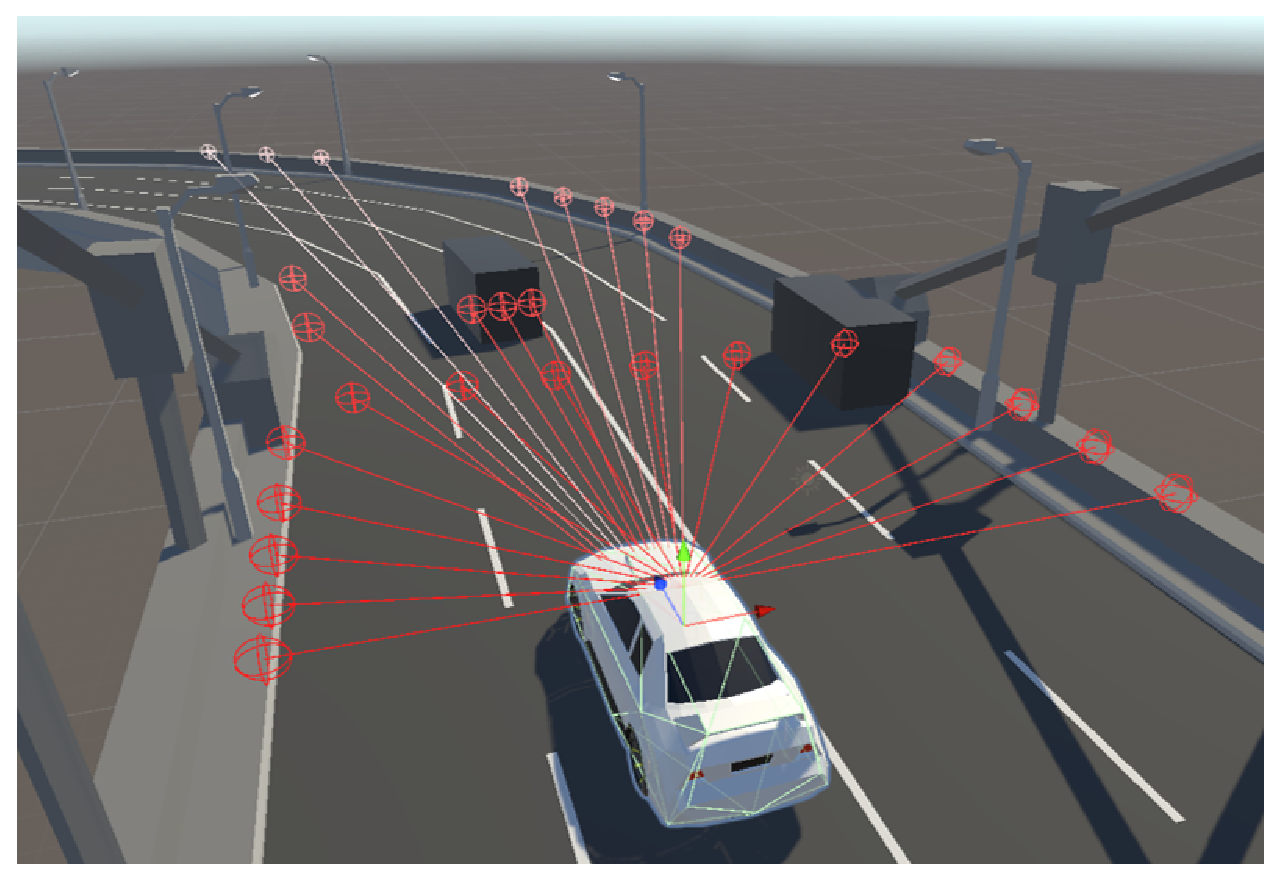
\includegraphics[width=0.8\textwidth]{figures/NonMovingObstacle.eps} % ここで図のファイル名とサイズを指定します
    \caption{静止している障害物} % 図のキャプション
    \label{fig:non-moving-obstacle} % 図への参照用ラベル
\end{figure}

\subsection{障害物の速度上昇}
さらに学習を進んで,エージェントは動的障害物,特にその速度を上げた障害物に対応することを学習する.障害物の数は2個から11個まで増やし,これによりエージェントはより複雑な環境下で運転する技術を習得する.より速い速度の障害物を回避するために,エージェントは予測と即時反応の両方が向上する.数が増えた障害物の学習を以下の図15に示す.
\begin{figure}[H]
    \centering
    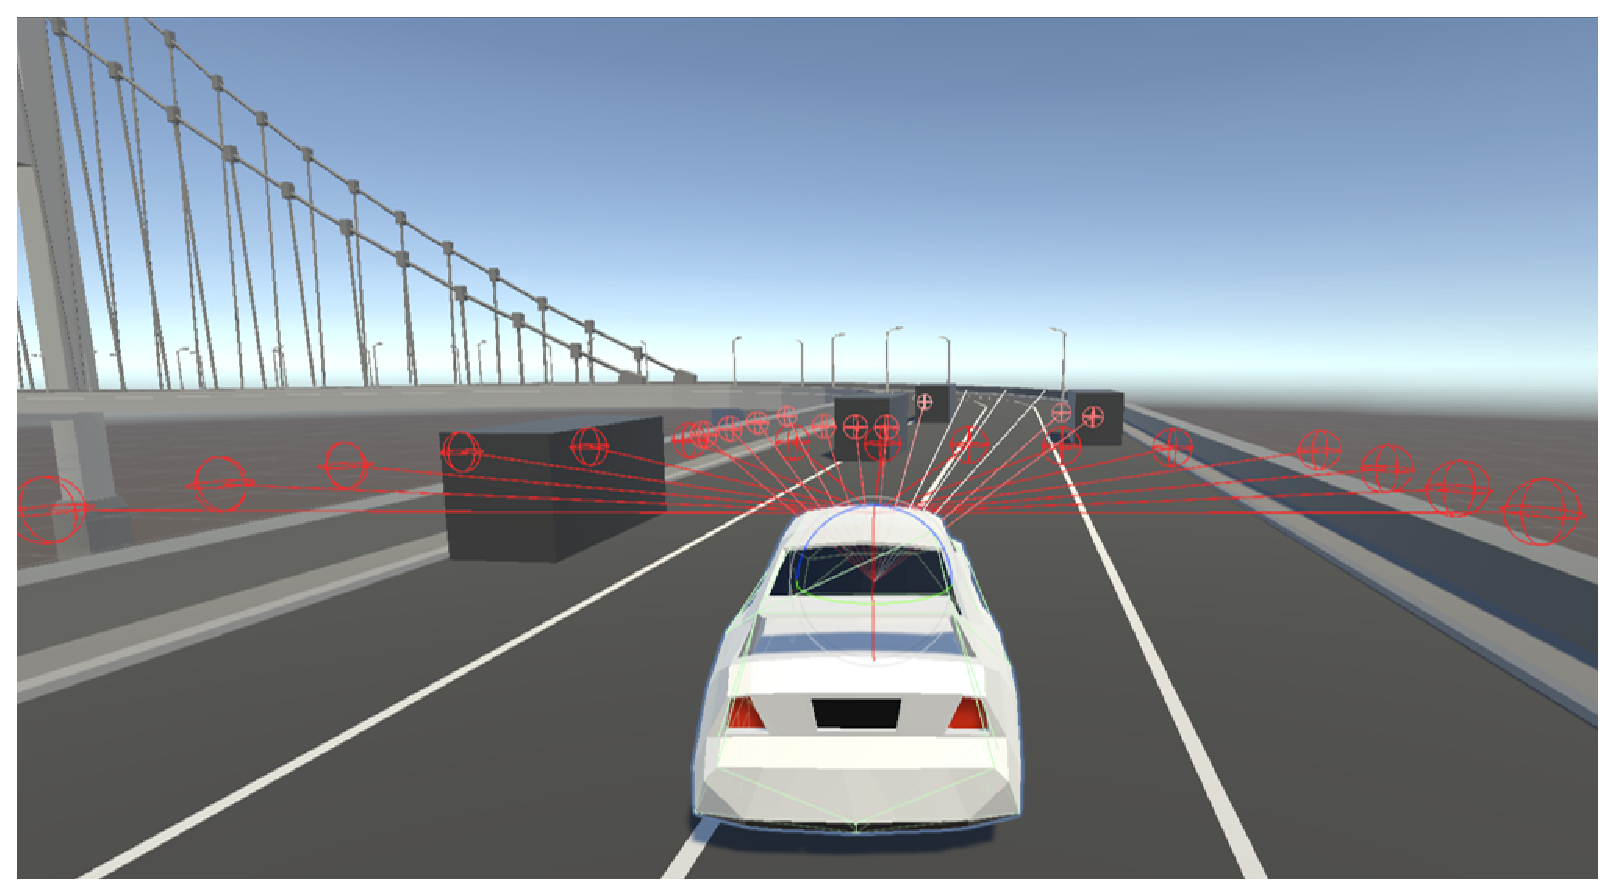
\includegraphics[width=0.8\textwidth]{figures/MovingObstacles.eps} % ここで図のファイル名とサイズを指定します
    \caption{障害物の速度上げと増えた数} % 図のキャプション
    \label{fig:moving-obstacles} % 図への参照用ラベル
\end{figure}

\subsection{四車線一方通行}
学習プロセスは次に,四車線一方通行のシナリオへと移る.この環境では,エージェントは追い越しを行うスキルを学習した.この段階での学習により,エージェントは一方通行の環境における複数車両の動きに適応する能力を示す.四車線一方通行の学習様子を以下の図16に示す.
\begin{figure}[H]
    \centering
    \includegraphics[width=0.8\textwidth]{figures/OneWayTraffic.eps} % ここで図のファイル名とサイズを指定します
    \caption{四車線一方通行} % 図のキャプション
    \label{fig:one-way-traffic} % 図への参照用ラベル
\end{figure}

\subsection{四車線対面通行}
最終的に,エージェントは四車線対面通行という,より高度な運転環境での学習を行う.対面通行のシナリオでは,エージェントは対向車線から来る車両と衝突を避けるための判断能力を高める必要があった.この環境での学習結果を一方通行の結果と比較することで,エージェントの適応能力と戦略の違いを明確になる.四車線対面通行の学習様子を以下の図17に示す.
\begin{figure}[H]
    \centering
    \includegraphics[width=0.8\textwidth]{figures/TwoWayTraffic.eps} % ここで図のファイル名とサイズを指定します
    \caption{四車線対面通行} % 図のキャプション
    \label{fig:two-way-traffic} % 図への参照用ラベル
\end{figure}

全体的に,本章はエージェントの学習プロセスを段階的に丁寧に説明している.各段階でのエージェントの目標とそれを達成するための方法,およびその結果が記述されている.報酬システムがエージェントの行動選択をどのように促し,学習を導いているかも効果的に示されている.

\subsection{学習結果}
\subsubsection{四車線一方通行の学習結果}
\begin{table}[H]
\centering
\caption{四車線一方通行の学習結果}
\label{tab:ippoutuukou}
\begin{tabular}{|c|c|c|c|c|}
\hline
\multirow{2}{*}{走行時間} & \multicolumn{4}{c|}{対向車なし} \\ \cline{2-5} 
                           & 50s & 100s & 150s & 200s \\ \hline
No. 1                       & 0   & 2    & 3    & 4    \\ \hline
No. 2                       & 0   & 1    & 3    & 2    \\ \hline
No. 3                       & 0   & 2    & 0    & 1    \\ \hline
No. 4                       & 1   & 0    & 3    & 3    \\ \hline
No. 5                       & 0   & 1    & 2    & 3    \\ \hline
No. 6                       & 0   & 0    & 2    & 5    \\ \hline
No. 7                       & 0   & 1    & 1    & 3    \\ \hline
No. 8                       & 0   & 2    & 2    & 2    \\ \hline
No. 9                       & 0   & 1    & 3    & 1    \\ \hline
No.10                      & 0   & 1    & 2    & 3    \\ \hline
平均                       & 0.1 & 1.1  & 2.1  & 2.7  \\ \hline
最高値                     & 1   & 2    & 3    & 5    \\ \hline
最低値                     & 0   & 0    & 0    & 1    \\ \hline
\end{tabular}
\end{table}
四車線一方通行のシナリオでの学習結果を示す表1は,各エピソードの走行時間(50秒,100秒,150秒,200秒)で10回実施したテストの結果である.グラフから分かるように,エピソードの時間が増えるにつれて平均衝突回数がわずかに増加する傾向が見られる.具体的には,50秒の走行では平均衝突回数が0.1回,200秒の走行では平均2.7回となっている.この結果から,走行時間が長くなるほど,車エージェントが直面するシナリオの数が増え,それに伴い衝突の可能性も高まることが示される.

このシナリオでは,最低値と最高値のデータを見ると,あるテストでは全く衝突が発生しないもあれば,最大で5回の衝突が発生する場合もあり,エージェントのパフォーマンスには個別の差があることが分かる.

\subsubsection{四車線対面通行の学習結果}
四車線対面通行についての学習結果を以下の表2に示す.
\begin{table}[H]
\centering
\caption{四車線対面通行の学習結果}
\label{tab:taimentuukou}
\begin{tabular}{|c|c|c|c|c|}
\hline
\multirow{2}{*}{走行時間} & \multicolumn{4}{c|}{対向車あり} \\ \cline{2-5} 
                           & 50s & 100s & 150s & 200s \\ \hline
No. 1                       & 0   & 2    & 3    & 6    \\ \hline
No. 2                       & 0   & 4    & 4    & 3    \\ \hline
No. 3                       & 0   & 1    & 3    & 3    \\ \hline
No. 4                       & 1   & 1    & 2    & 4    \\ \hline
No. 5                       & 0   & 2    & 4    & 6    \\ \hline
No. 6                       & 0   & 2    & 4    & 2    \\ \hline
No. 7                       & 0   & 1    & 1    & 2    \\ \hline
No. 8                       & 1   & 2    & 5    & 3    \\ \hline
No. 9                       & 0   & 1    & 3    & 3    \\ \hline
No.10                      & 1   & 2    & 4    & 4    \\ \hline
平均                       & 0.3 & 1.8  & 3.3  & 3.6  \\ \hline
最高値                     & 1   & 4    & 5    & 6    \\ \hline
最低値                     & 0   & 1    & 1    & 2    \\ \hline
\end{tabular}
\end{table}
表2を見ると,四車線対面通行のシナリオでは,一方通行のシナリオと比較して,全体的に平均衝突回数が高くなっている.特に200秒の走行では平均衝突回数が3.6回に達しており,これは対面通行が一方通行よりもエージェントにとって運転が難しい状況であることを示している.エージェントは自車線の障害物だけでなく,対向車線から接近する障害物にも対応する必要がり,対向車の有無のシナリオにより予測すべき変数が変化するため,より良い運転方法を学習することが難しくなることに起因すると考えられる.

\subsection{考察}
最終的な学習結果から,四車線一方通行のシナリオではエージェントが比較的良い成果を示した一方で,対面通行のシナリオにおいてはまだ改善の余地があると考えられる.\\









\newpage
\section{おわりに}
本研究では,Unityでのゲーム環境の構築と深層強化学習を駆使した自動運転AIを作成することができたが,高速で走る暴走する側を作ってしまったので,元々の安全運転という目的を実現することはできなかった.今後,この研究を改善し,将来的に暴走する側ではなく,ちゃんとした高速で判断力の高いモデルを作成していきたいと思っている.\\

\noindent
\textbf{今後の課題}\\
これらのモデル,特に対面通行のシナリオを改善するためには,いくつかの方法が考えられる.一つの提案として,道路を自車線エリアと対向車線エリアの2つに分け,自車線エリアにいる間は小さな一定の報酬を,対向車線にいる間は小さな一定のペナルティを与えるという方法がある.このアプローチにより,学習過程でエージェントが自車線の走行を優先することの重要性を理解し,対向車線への進入を避けるよう学習することが期待される.


\titleformat{\section}{\normalfont\Large\bfseries}{}{0em}{}

\newpage
\section*{謝辞}
\addcontentsline{toc}{section}{謝辞}

本研究を進めるにあたり,初めから丁寧にご指導いただいた越野先生に深く感謝いたします.3年生で編入して以来,先生には大変お世話になりました.留学生としてこのクラスに参加する際,教室や研究室の皆さんと上手く交流できるか,先生と楽しい会話ができるかという不安がありました.しかし,そのような心配は全く必要ありませんでした.越野先生は,常に研究に関する豊富なアイデアを提供してくださり,趣味や面白い話も共有してくださいました.人生相談にも乗っていただき,編入試験の際には面接の練習や,自分の長所と短所を見つけるお手伝いもしてくれました.この3年間,先生には本当に感謝しています.また,一緒に頑張っていた研究生の仲間,佳山君,萬年君,加藤君,宇野君のおかげで1年間の研究活動を楽しく進めることができ,本当にありがとうございました.
研究室の雰囲気も常に明るく,孤立することなく温かい研究室の一員として過ごすことができました.

この1年間で,研究だけでなく,将来に向けた夢や目標に対するモチベーションも格段に高まり,自己成長を実感するとても充実した年となりました.これからも,大学,大学院,そして就職という新たなステップに自信を持って挑み,留学生や外国人として日本や様々な国の架け橋となり,前向きな姿勢で取り組んでいきたいと思います!


\newpage
\printbibliography[title=参考文献]
\addcontentsline{toc}{section}{参考文献}

\end{document}
